\chapter*{Samenvatting}
\label{cha:Samenvatting}
\addcontentsline{toc}{chapter}{Samenvatting}
% Let op! geen verwijzingen naar paragrafen in de samenvatting. Hij moet zelfstandig leesbaar zijn

Voor de ontwerpwedstrijd van de studie Werktuigbouwkunde moesten alle eerstejaarsstudenten een pakkethondje ontwerpen. Dit pakkethondje moest een pakketje van een verhoging kunnen aannemen, daarmee over een parcours met een talud en een zelfgekozen hindernis. De zelfgekozen hindernis wordt gekozen op basis van moeilijkheid, wat extra punten oplevert. Ze zijn gemaakt van opsluitbanden en hebben een individuele afmeting van 55x145x1000 mm. Dit rapport beschrijft de het ontwerpproces, de verschillende concepten en het uiteindelijke gekozen ontwerp.

Op basis van het programma van eisen zijn er verschillende deeloplossingen in een morfologische kaart gezet. Door combinaties van deze deeloplossingen te maken zijn er 4 kansrijke concepten bedacht, welke verder zijn uitgewerkt.

Het eerste concept is de Mantis car. De Mantis car werkt door middel van grijphaken die gebaseerd zijn op hetzelfde idee als de poten van een sprinkhaan, zie \cref{fig:deeloplossing_mantis2}. De grijphaken zijn verbonden met een as, welke aangedreven wordt door een elektromotor. Hiermee kunnen de verschillende taluds worden overwonnen doordat het concept zichzelf omhoog trekt. Het voordeel van de Mantis car is dat het makkelijk te construeren is. Het nadeel is de stabiliteit van het pakketje. Deze komt tijdens het overwinnen van de taluds schuin te staan en dit kan verschillende problemen veroorzaken.

\begin{figure}[h]
    \centering
    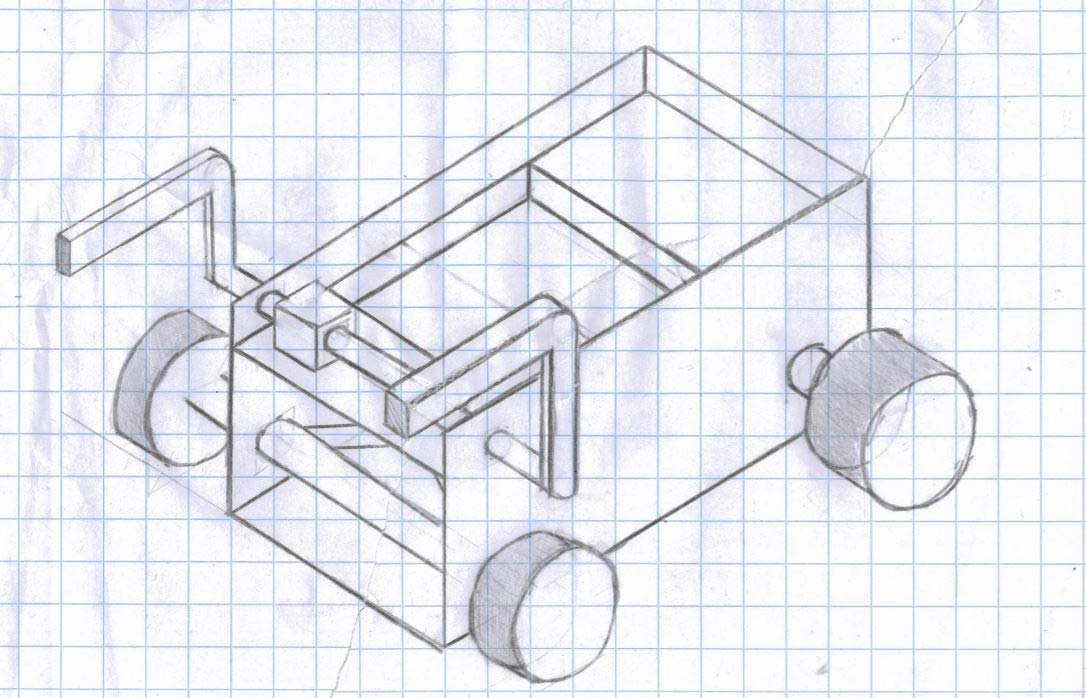
\includegraphics[width = 80mm]{04_idee_ontwikkeling/deeloplossing_mantis.JPG}
    \caption{Concept 1, de Mantis car}
    \label{fig:deeloplossing_mantis2}
\end{figure}

Het tweede concept is de Uitschuiver. De Uitschuiver heeft 2 delen welke afzonderlijk kunnen worden ingetrokken en uitgeschoven, zie \cref{fig:isom_uitschuiver2}. De Uitschuiver heeft ook inklapbare pootjes, welke kunnen worden ingetrokken. Wanneer deze worden ingetrokken kan het voorste deel van de Uitschuiver over het talud heen worden geschoven, en zo kan het obstakel worden overwonnen. Het zwaartepunt kan worden veranderd door het pakketje heen en weer te schuiven. Een voordeel van dit concept is dat de werking voorspelbaar is. Dit omdat het talud niet wordt aangeraakt bij dit concept en het model niet wordt belast op krachten die niet van tevoren te voorspellen zijn. Een nadeel is de maakbaarheid, omdat het uitschuifmechanisme in combinatie met de het schuiven van het pakketje een gecompliceerd systeem is.

\begin{figure}[!htp]
    \centering
    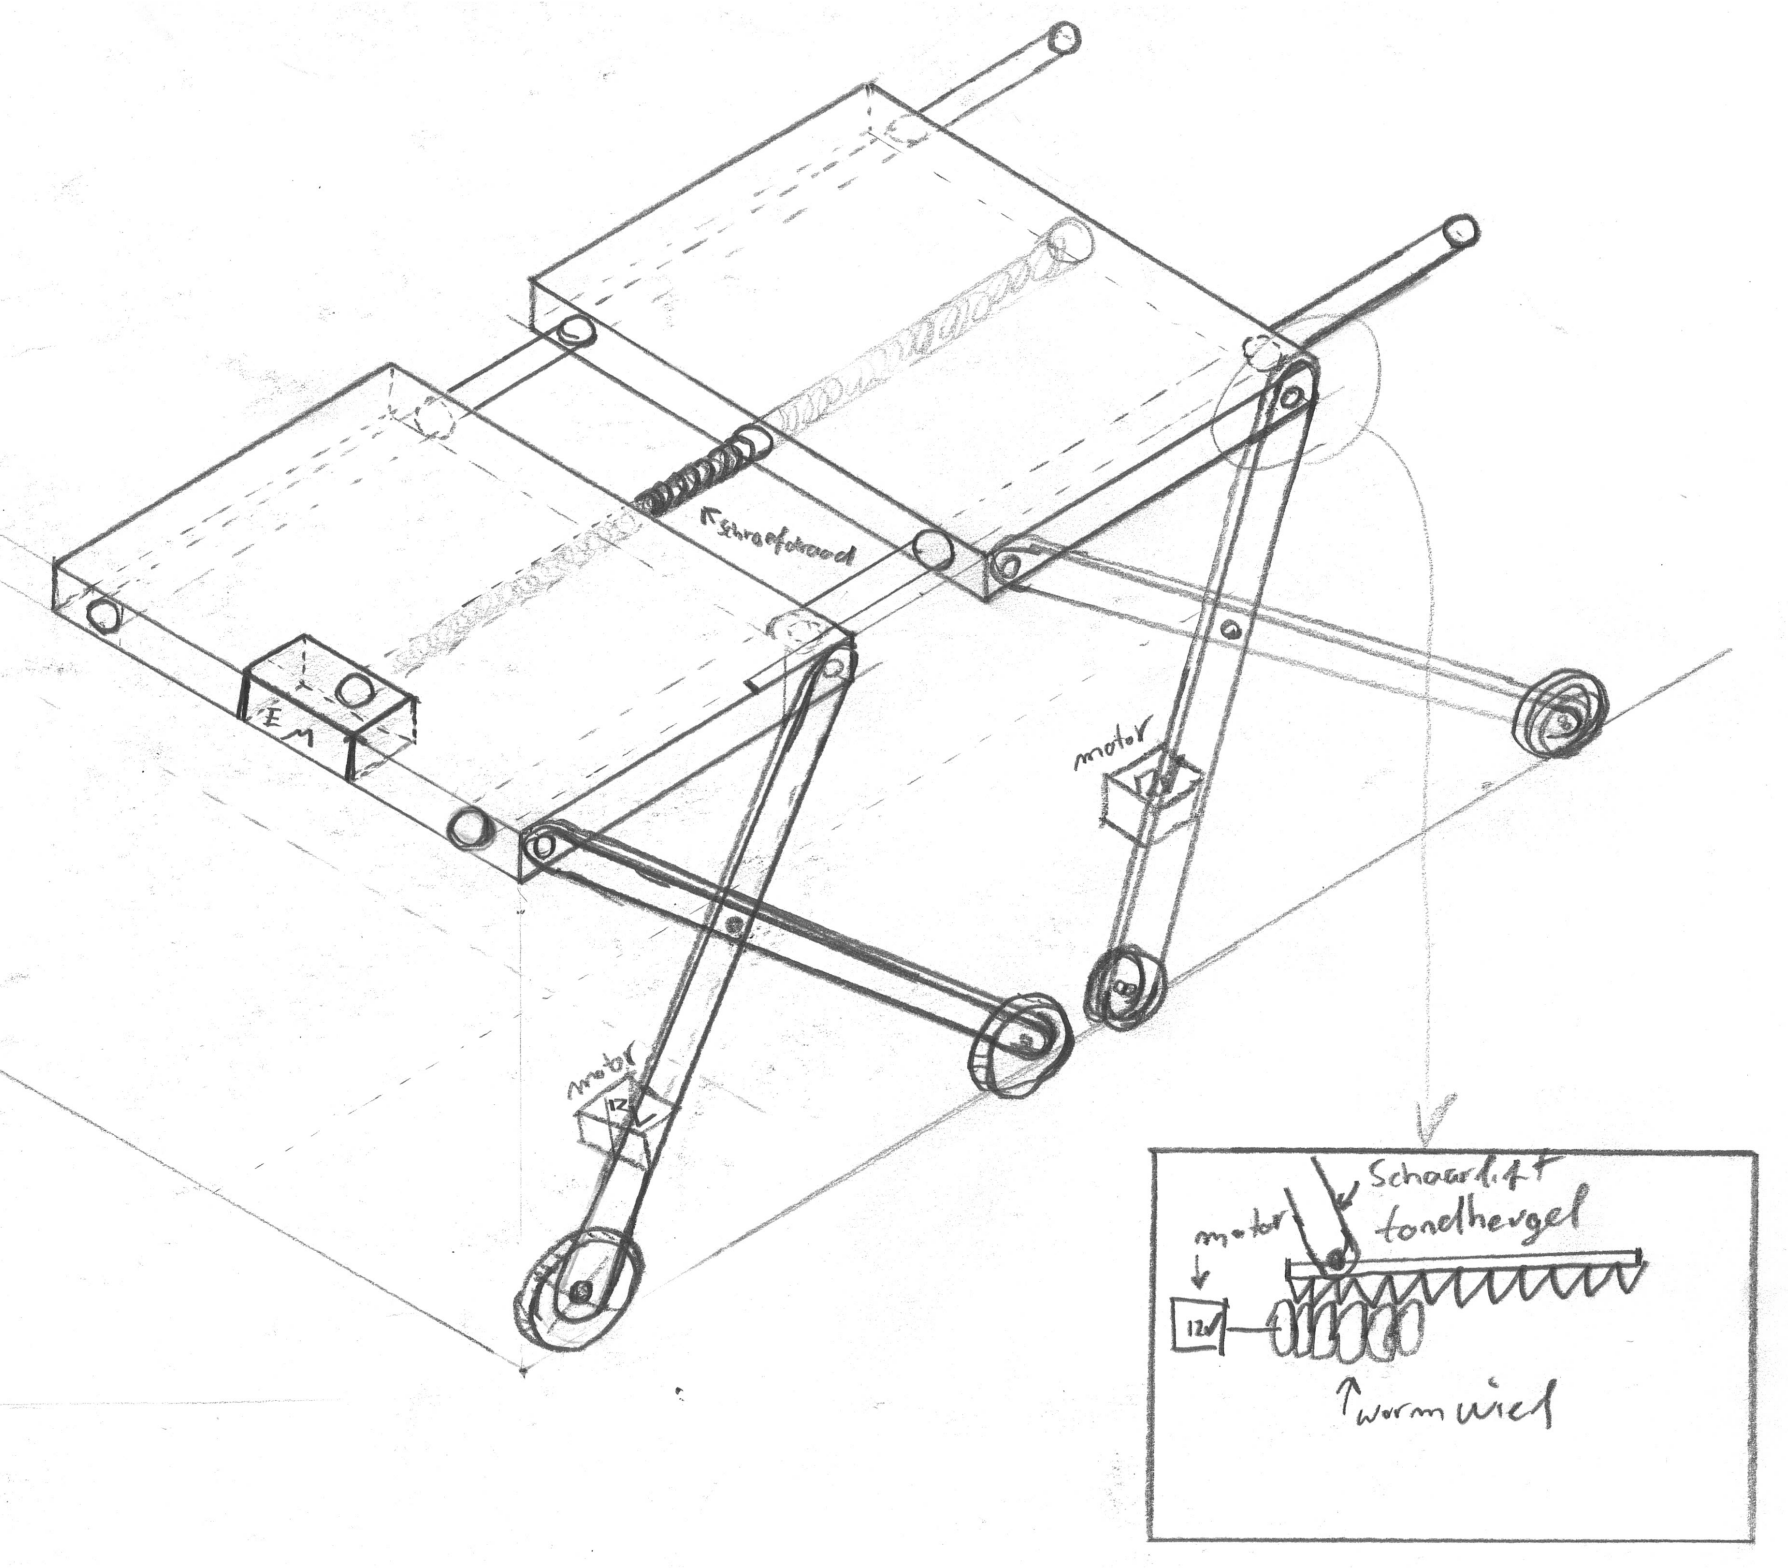
\includegraphics[width=80mm]{04_idee_ontwikkeling/isom_uitschuiver.png}
    \caption{Concept 2, de uitschuiver}
    \label{fig:isom_uitschuiver2}
\end{figure}

Het derde concept is de Inklapper. Zoals de naam al verraad klappen de pootjes en de schaarlift een voor een in waardoor de Inklapper over het obstakel heen kan rijden zonder het obstakel ook echt aan te raken, zie \cref{fig:inklapper2} en \cref{fig:inklapper_schuif2}. Bij dit concept kan het pakketje ook heen en weer worden geschoven om het zwaartepunt te veranderen. Het voordeel hiervan is dat het makkelijker te maken is met dezelfde voordelen als de Uitschuiver. Een nadeel is dat de wielen relatief veel bewegingsvrijheid hebben. 

\begin{figure}[H]
    \centering
    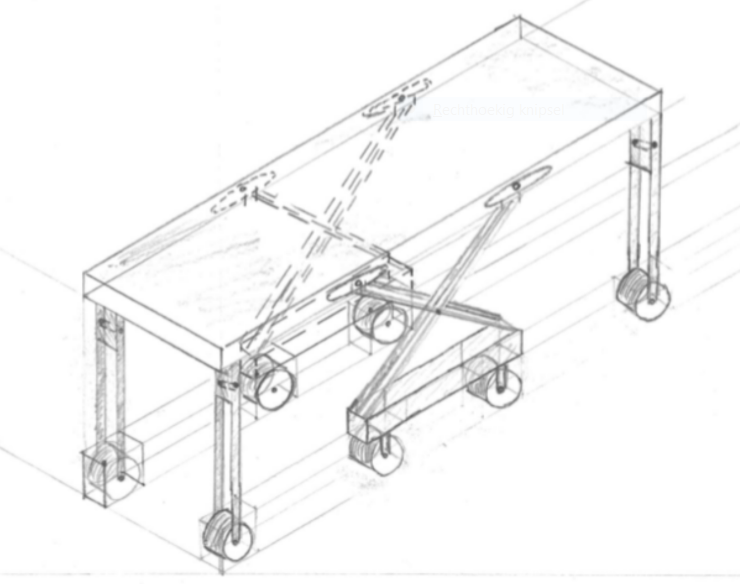
\includegraphics[width = 80mm]{Foto_inklapper.PNG}
    \caption{Concept 3, De inklapper, het in klapmechanisme}
    \label{fig:inklapper2}
\end{figure}

\begin{figure}[H]
    \centering
    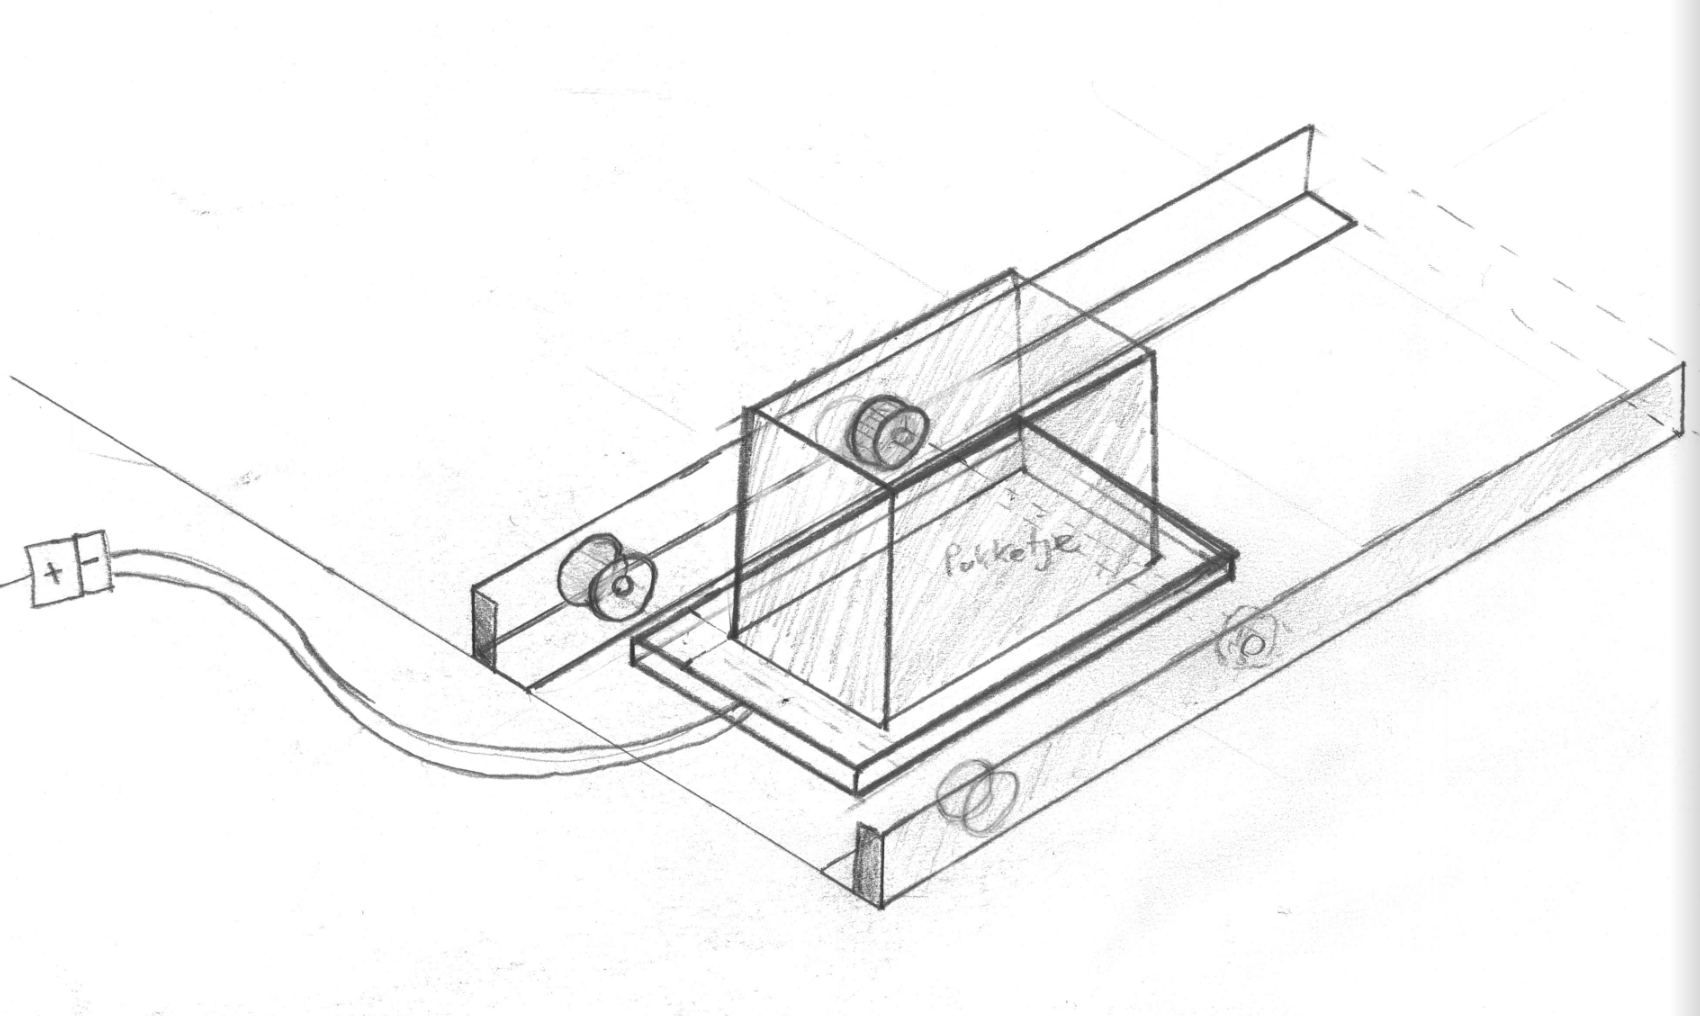
\includegraphics[width = 80mm]{04_idee_ontwikkeling/detail_uitschuiver.png}
    \caption{Concept 3, De inklapper, het schuifmechanisme}
    \label{fig:inklapper_schuif2}
\end{figure}

Het vierde concept is de Vierpoter, de Vierpoter heeft 4 poten en heeft geen variabel zwaartepunt, waardoor er met genoeg afstand tussen de wielen over het obstakel heen kan worden gestapt. De assen die aan de bovenkant te zien zijn in \cref{fig:vierpoter_totaal2} zijn er om het pakketje te ontvangen Het nadeel van de grote afstand tussen de wielen is dat het gehele ontwerp 3 keer zo lang moet worden als het obstakel en zou het in 3 delen demonteerbaar moeten zijn om te voldoen aan de eisen van de ontwerpopdracht. Het voordeel is dat het zwaartepunt niet hoeft te worden verplaatst en daardoor is het een makkelijk ontwerp om te maken.

\begin{figure}[h]
    \centering
    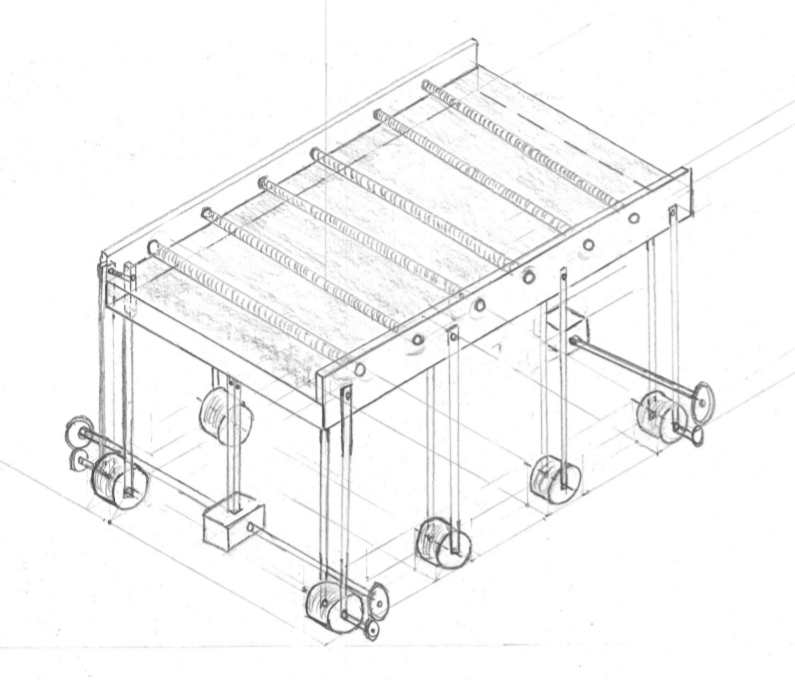
\includegraphics[width = 80mm]{04_idee_ontwikkeling/Foto_vierpoter.PNG}
    \caption{Concept 4, de vierpoter}
    \label{fig:vierpoter_totaal2}
\end{figure}
\vspace{\baselineskip}
Met de gewogen criteria methode is er uiteindelijk gekozen voor een combinatie van de Inklapper met de Vierpoter, genaamd de 'Driepoot'. De Driepoot neemt de hindernisbaan op dezelfde manier als de Vierpoter, maar heeft schaarliften onderin i.p.v. inklapbare poten. Het gebruik van schaarliften heeft twee voordelen: het is gemakkelijker te maken en het is stabieler. Het gewicht van de driepoot is 10 kg in totaal. In \cref{fig:uiteindelijke_concept} is het totaalconcept afgebeeld.

\begin{figure}[h]
    \centering
    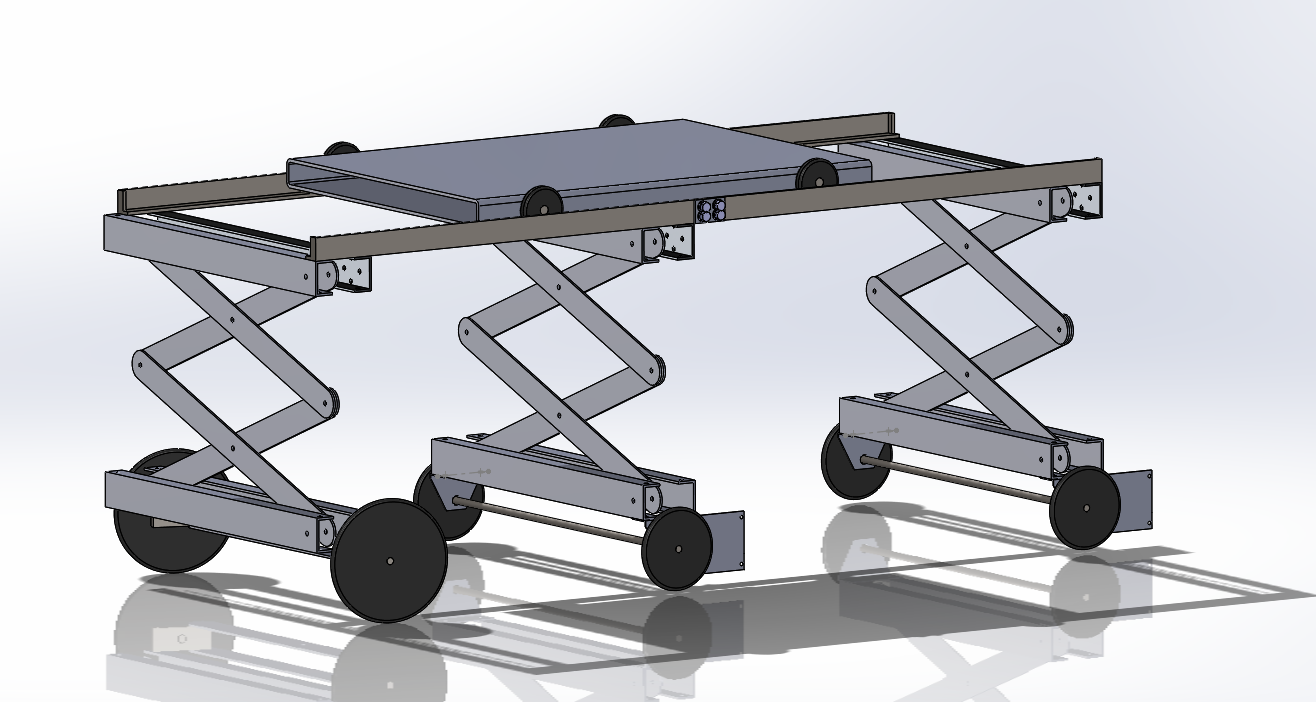
\includegraphics[width = 100mm]{04_gekozenconcept/eindconcept.png}
    \caption{Gekozen concept, inklapper (uitgewerkt)}
    \label{fig:uiteindelijke_concept}
\end{figure}